\usetikzlibrary{calc}


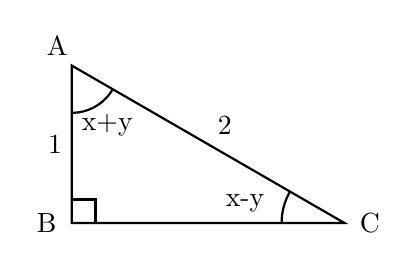
\begin{tikzpicture}[scale=1]

    % Define the vertices of the right-angled triangle
    % Using coordinates that match the 1:sqrt(3):2 ratio of a 30-60-90 triangle
    \coordinate (B) at (0,0);
    \coordinate (C) at (3.464, 0); % 2 * sqrt(3) scaled down to match height 2
    \coordinate (A) at (0, 2);

    % Draw the main triangle
    \draw[thick] (A) -- (B) -- (C) -- cycle;

    % Draw the right-angle symbol at B
    \draw[thick] (0.3, 0) -- (0.3, 0.3) -- (0, 0.3);

    % Draw the angle arcs
    % Arc at A (between AB at 270 degrees and AC at 330 degrees)
    \draw[thick] (A) ++(270:0.6) arc (270:330:0.6);
    
    % Arc at C (between CB at 180 degrees and CA at 150 degrees)
    \draw[thick] (C) ++(180:0.8) arc (180:150:0.8);

    % Add labels for the vertices
    \node[above left, xshift=2pt] at (A) {A};
    \node[left, xshift=-2pt] at (B) {B};
    \node[right, xshift=2pt] at (C) {C};

    % Add side length measurements
    \node[left] at (0, 1) {1};
    \node[above right] at (1.732, 1) {2};

    % Add angle expressions inside the triangle
    \node at (0.45, 1.25) {x+y};
    \node at (2.2, 0.25) {x-y};

\end{tikzpicture}